\section{\ocaml implementation}
\label{sec:ocaml}

\lstset{language=[Objective]Caml}

In addition to the \haskell implementation, we implemented our language generator
in \ocaml.
The \ocaml version only implements the ``latest'' version of the
algorithm with a segmented representation, and fast backward lookup for concatenation and star.
% One of the goal of this implementation was to test
% pure \ocaml regular expression libraries such as ocaml-re\footnote{\url{https://github.com/ocaml/ocaml-re}} and
% mulet\footnote{\url{https://github.com/let-def/mulet}}. 
The main goal of this implementation was to experiment with strictness
and various data-structure for segments. 
The key idea is that, since each segment contains only words of the same length,
the internal order does not matter. We simply need a data structure
supporting (fast) power series operations.
In order to test this, we implemented our algorithm as a functor whose signature
is shown in \autoref{code:sigs}.
Our functor takes as argument two data-structures: words and segments.
This way, we can easily test numerous representation without changing
our code. This also gave us the opportunity to find the ``minimal'' operations
needed to implement our algorithm, which we now describe.

\begin{figure}[b]
  \centering
  \begin{subfigure}{0.44\linewidth}
\begin{lstlisting}[basicstyle=\scriptsize\ttfamily]
module type SEGMENT = sig
  type elt (** Elements *)
  type t (** Segments *)

  val empty : t
  val is_empty : t -> bool
  val return : elt -> t

  (** Set operations *)
  val union : t -> t -> t
  val inter : t -> t -> t
  val diff : t -> t -> t

  (** Product and append elements *)
  val append: t -> t -> t

  (** n-way merge *)
  val merge : t list -> t

  (** Import a list *)
  val of_list : elt list -> t

  (** Export elements *)
  val iter : t -> (elt -> unit) -> unit

  (** For transient data-structures *)
  val memoize : t -> t
end
\end{lstlisting}
    \caption{Necessary operation on segments}
    \label{code:sigs:segment}
  \end{subfigure}~
  \begin{subfigure}{0.57\linewidth}
\begin{lstlisting}[basicstyle=\scriptsize\ttfamily]
module type WORD = sig
  type char
  type t
  val empty : t
  val singleton : char -> t
  val append : t -> t -> t
end
\end{lstlisting}
    \caption{Necessary operation on words}
    \label{code:sigs:word}
\begin{lstlisting}[basicstyle=\scriptsize\ttfamily]
module Regenerate
    (Word : WORD)
    (Segment : Segments.S with type elt = Word.t)
: sig
  type lang = Segment.t stream
  val gen : 
    sigma:Segment.t -> C.t regex -> lang
  val iter : lang -> (Word.t -> unit) -> unit
end
\end{lstlisting}
    \caption{Language generation as a functor}
    \label{code:sigs:regen}
  \end{subfigure}
  \caption{Signatures of the language generator}
  \label{code:sigs}
\end{figure}

\paragraph{Character and Words}

The signature for words in shown in \autoref{code:sigs:word}.
Surprisingly few operations are needed for words: Indeed, we mostly requires the ability to build the empty word (for \code{One}),
words of one char (for \code{Atom}) and to append words
with each others.
Notably, we do not require an ordering on words: as said above, comparison between words is not required by the core algorithm and is simply a matter for the segment
data structure.
We also do not require a \code{length} operation: since words are always
classified in the appropriate segments, their length is simply the index
of the segment.

In practice, such a signature is easily satisfied by the \ocaml \code{string}
type (\ie arrays of bytes), arrays or lists of characters, or ropes. The
type of individual characters is completely unrestricted.

\paragraph{Segments}

The signature for segments is shown in \autoref{code:sigs:segment}.
The main requirement is the support for the various operations on power series described in
\autoref{sec:ordered-enumeration}.
For the set operations, we require
\code{union}, \code{inter} and \code{inter} functions.
%
The product described in \autoref{eq:1} is decomposed in two parts:
\begin{itemize}
\item  An \code{append} function which implement $U_i V_{n-i}$. It takes the
  product of two segments and append their elements two by two.
\item A \code{merge} operation which takes the union of an arbitrary number
  of segments. This allows to collect the various segments obtained
  with \code{append}.
\end{itemize}
%
Since our goal is to experiment with various data structures, we want to allow
ourselves to use implementations that are transient by default. We thus require
a \code{memoize} function that will avoid recomputing segments accessed multiple times, which is the case for the concatenation of languages.
%
Finally, we also need ways to import and export the elements of a segment, using \code{of_list} and \code{iter}.

\subsection{Core algorithm}

The core algorithm is very similar to the Haskell version. The power series
is implemented using a thunk-list in the style of \citet{DBLP:conf/cpp/Pottier17}:

\begin{lstlisting}
type 'a node =
  | Nil
  | Cons of 'a * 'a stream
type 'a stream = unit -> 'a node
\end{lstlisting}

A stream is represented by a function which takes a unit argument and returns
a node. A node, in turn, is either \code{Nil} or a \code{Cons} of an
element and the tail of the stream. The empty stream, for instance, is
represented as \code{fun () -> Nil}.
This representation has multiple advantages\footnote{See \url{https://github.com/ocaml/ocaml/pull/1002} for a (very) long discussion on the topic.}: it is lazy, fast, lightweight and almost as easy to manipulate as regular lists.
It gives us a very natural representation for languages represented as power series:
\begin{lstlisting}[numbers=none]
type lang = Segment.t stream
\end{lstlisting}

The rest of the implementation follow similarly to the \haskell one. For instance
here is the implementation of the union of languages:
\begin{lstlisting}
let rec union s1 s2 () = match s1(), s2() with
  | Nil, x | x, Nil -> x
  | Cons (x1, next1), Cons (x2, next2) -> 
    Cons (Segment.union x1 x2, union next1 next2)
\end{lstlisting}
Note the presence of unit arguments, \code{()}, which allow to control the
evaluation of the stream. With this definition, \code{union s1 s2} will not lead
to any evaluation until \code{()} is provided. This ensures that the stream is
properly lazy.

The concatenation of languages demonstrate how the main algorithm can
be expressed once the segment operation have been abstracted:.
In order to build $U \cdot V$, we first build the $n$th term
$(U \cdot V)_n = \bigcup_{i=0}^n U_i V_{n-i}$.
We use both \code{Segment.append} to implement the product
of segment and the concatenation of words, and \code{Segment.merge} to merge
all the resulting subterms.
\begin{lstlisting}
let term_of_length map1 map2 n =
  let combine_segments i =
    Segment.append (IntMap.find i map1) (IntMap.find (n - i) map2)
  in
  List.(range 0 n) |> List.rev_map combine_segments |> Segment.merge
\end{lstlisting}

We then collect all the terms by synchronized recursion over the power series $U$
and $V$:
\begin{lstlisting}
let rec collect n map1 map2 seq1 seq2 () = match seq1 (), seq2 () with
  | Cons (segm1, seq1), Cons (segm2, seq2) ->
    let map1 = IntMap.add n (Segment.memoize segm1) map1 in 
    let map2 = IntMap.add n (Segment.memoize segm2) map2 in
    Cons (term_of_length map1 map2 n, collect (n+1) map1 map2 seq1 seq2)
\end{lstlisting}

Note the use of \code{IntMap} to gain fast access to smaller
segments that have already been computed. Since such segments will be accessed
multiple time, we use \code{memoize} to avoid computing them again and again.
The use of functional maps here is sufficient: the size of map is equal
to the maximum word length, which should not be excessively big.

Finally, we initialize \code{collect} with empty maps.
\begin{lstlisting}[numbers=none]
let concatenate = collect 0 IntMap.empty IntMap.empty
\end{lstlisting}

\subsection{Data structure}

We have implemented our language generator parameterized by segments, we can now
experiment various data-structures for segments. We present various
potential implementation before comparing their performances.

\subsubsection{Ordered streams}

The \haskell implementation presented in \autoref{sec:ordered-enumeration}
represent segments as ordered enumerations. We can use
the same representation in \ocaml thanks to the \code{stream} datatype.
\begin{lstlisting}[numbers=none]
type t = elt stream
\end{lstlisting}

Since we use an order, we require a comparison function on elements.
We also need an \code{append} functions on word. We summarize these requirement
with the \code{OrderedMonoid} signature.
We can the define the \code{ThunkList} functor shown in \autoref{code:thunklist}.
We omit most of the function, as they can trivially implemented in a way

\begin{figure}
  \centering
\begin{lstlisting}
module type OrderedMonoid = sig
  type t
  val compare : t -> t -> int
  val append : t -> t -> t
end
module ThunkList (Elt : OrderedMonoid) : SEGMENTS with type elt = Elt.t
\end{lstlisting}
  \caption{Signature for \texttt{ThunkList}}
  \label{code:thunklist}
\end{figure}

The rest of the implementation is straightforward. For example, here is the
\code{append} function, where \code{>>=} is bind (or \code{concatMap})
and \code{>|=} is map.

\begin{lstlisting}
let append l1 l2 =
  l1 >>= fun x -> l2 >|= fun y -> Elt.append x y
\end{lstlisting}

The n-way merge is implemented using a priority heap which hold pairs composed
of the head of a stream and its tail. When a new element is required in the
merged stream, we pop the top element of the heap, deconstruct
the tail and insert it back in the heap.

\begin{lstlisting}
let merge l =
  let cmp (v1,_) (v2,_) = K.compare v1 v2 in
  let merge (x1, s1) (_, s2) = (x1, s1@s2) in
  let push h s =
    match s() with Nil -> h | Cons (x, s') -> Heap.insert h (x, [s'])
  in
  let h0 = List.fold_left push (Heap.empty ~cmp ~merge) l in
  let rec next heap () =
    if Heap.is_empty heap then Nil else begin
      let (x, seq), heaps = Heap.pop heap in
      let new_heap = List.fold_left push heaps seq in
      Cons (x, next new_heap)
    end
  in
  next h0
\end{lstlisting}

\subsubsection{Transience and Memoization}

During concatenation and star, we iterate over segments multiple time.
Unfortunately thunk lists are transient: iterating multiple time over the same list
will compute it again. To offset this, we can implement memoization
over thunk lists by pushing the elements in a growing vector as they are
computed:
\begin{lstlisting}
let memoize f =
  let r = CCVector.create () in
  let rec f' i seq () =
    if i < CCVector.length r
    then CCVector.get r i
    else 
      let l = match seq() with
        | Nil -> Nil
        | Cons (x, tail) -> Cons (x, f' (i+1) tail)
      in
      CCVector.push r l;
      l
  in
  f' 0 f
\end{lstlisting}

Such a memoization function incurs a linear cost on streams. To test
if this operation is worthwhile we implemented two modules:
\code{ThunkList} where memoization is the identity and \code{ThunkListMemo}
with the implementation above.

\subsubsection{Lazy lists}

\ocaml also supports regular lazy lists using the builtin \code{lazy} keyword:

\begin{lstlisting}
type 'a node =
  | Nil
  | Cons of 'a * 'a lazylist
type 'a lazylist = 'a node Lazy.t
\end{lstlisting}

We hence implemented the \code{LazyList} functor which is identical to the
\code{ThunkList} but uses lazy lists.

\subsubsection{Strict sets}

Since the main operation for segments are set operations, it is natural to
expect sets to perform well. We implemented segments as sets
of words using \ocaml builtin \code{Set} module. \ocaml sets are implemented
using binary trees with an imbalance of at most one.
The only operations not implemented by \ocaml's standard library are
the n-way merge and the cartesian production which are easily implemented with
standard functions such as fold and union.

\subsubsection{Tries}

Tries are prefix trees where each branch is labeled with
a character. A word is considered to belong to the trie if it is possible to
follow its character and reach a value. Our problem seem very suitable to tries:
\begin{itemize}
\item All words in a segment are of the same length and can thus never be prefixes
  of each other. This mean that we can use tries where values are only
  at the leaf.
\item The \code{append} operation on tries can simply implemented by
  grafting the second trie in all the leafs of the first one.
\end{itemize}

\TODO{}

\subsection{Results}

We followed the same benchmarking methodology than for the \haskell
version in \autoref{sec:bench}. Benchmark for various data-structures
for regular expressions \verb/a*/, \verb/(ab*)*/ and \verb/~(a*)b/ are
presented in \autoref{fig:bench:ocaml:all}.

\begin{figure}
  \centering
  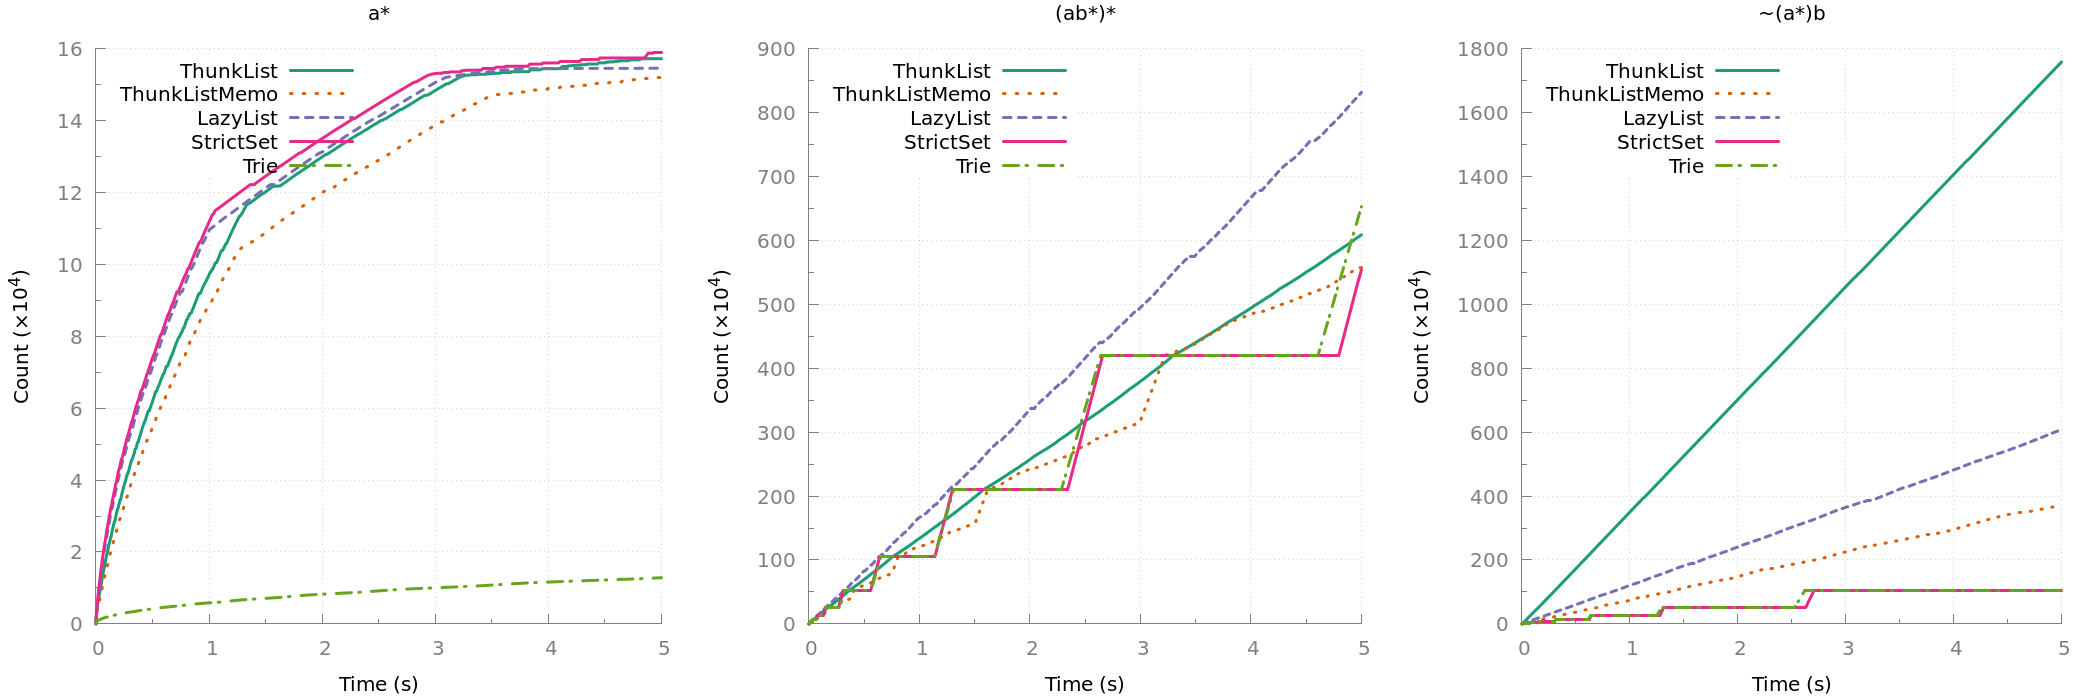
\includegraphics[width=\linewidth]{measure/ocaml_all.png}
  \caption{Benchmark for the \ocaml implementation with various data-structures.}
  \label{fig:bench:ocaml:all}
\end{figure}


%%% Local Variables:
%%% mode: latex
%%% TeX-master: "main"
%%% End:
